\documentclass[xcolor=dvipsnames]{beamer}
\usepackage[T1]{fontenc}
\usepackage[utf8]{inputenc}
\usepackage[english,slovak]{babel}

\usepackage{amsmath}
\usepackage{amsthm}
\usetheme{Pittsburgh}
\useoutertheme{shadow}

\usepackage{graphicx}
\usepackage{caption}
\usepackage{subcaption}

\usepackage[]{algorithm2e}
\usepackage{listings}
 \setbeamercovered{transparent}
 \usepackage{cuted}
\usepackage[export]{adjustbox}
\usepackage{mathtools}

\usepackage{lipsum}
\usepackage{verbatim}
\usepackage{transparent}
\usepackage{framed}
\usepackage{xcolor}

\newcommand\Wider[2][3em]{%
\makebox[\linewidth][c]{%
  \begin{minipage}{\dimexpr\textwidth+#1\relax}
  \raggedright#2
  \end{minipage}%
  }%
}




\iftrue

\usetheme{Warsaw}

\setbeamercolor{normal text}{fg=white,bg=black!90}
\setbeamercolor{structure}{fg=white}

\setbeamercolor{alerted text}{fg=red!85!black}

\setbeamercolor{item projected}{use=item,fg=black,bg=item.fg!35}

\setbeamercolor*{palette primary}{use=structure,fg=structure.fg}
\setbeamercolor*{palette secondary}{use=structure,fg=structure.fg!95!black}
\setbeamercolor*{palette tertiary}{use=structure,fg=structure.fg!90!black}
\setbeamercolor*{palette quaternary}{use=structure,fg=structure.fg!95!black,bg=black!80}

\setbeamercolor*{framesubtitle}{fg=white}

\setbeamercolor*{block title}{parent=structure,bg=black!60}
\setbeamercolor*{block body}{fg=black,bg=black!10}
\setbeamercolor*{block title alerted}{parent=alerted text,bg=black!15}
\setbeamercolor*{block title example}{parent=example text,bg=black!15}

\fi



%-------------------------------------------------------------------------------------
\title{\color{white} \bf Reinforcement learning}
\author{\color{white} Michal CHOVANEC, PhD}


%\setbeamertemplate{footline}[frame number]{}
\setbeamertemplate{navigation symbols}{}


\date[EURP]{}
\begin{document}

{
    \usebackgroundtemplate
    {
        \vbox to \paperheight{\vfil\hbox to \paperwidth{\hfil

        {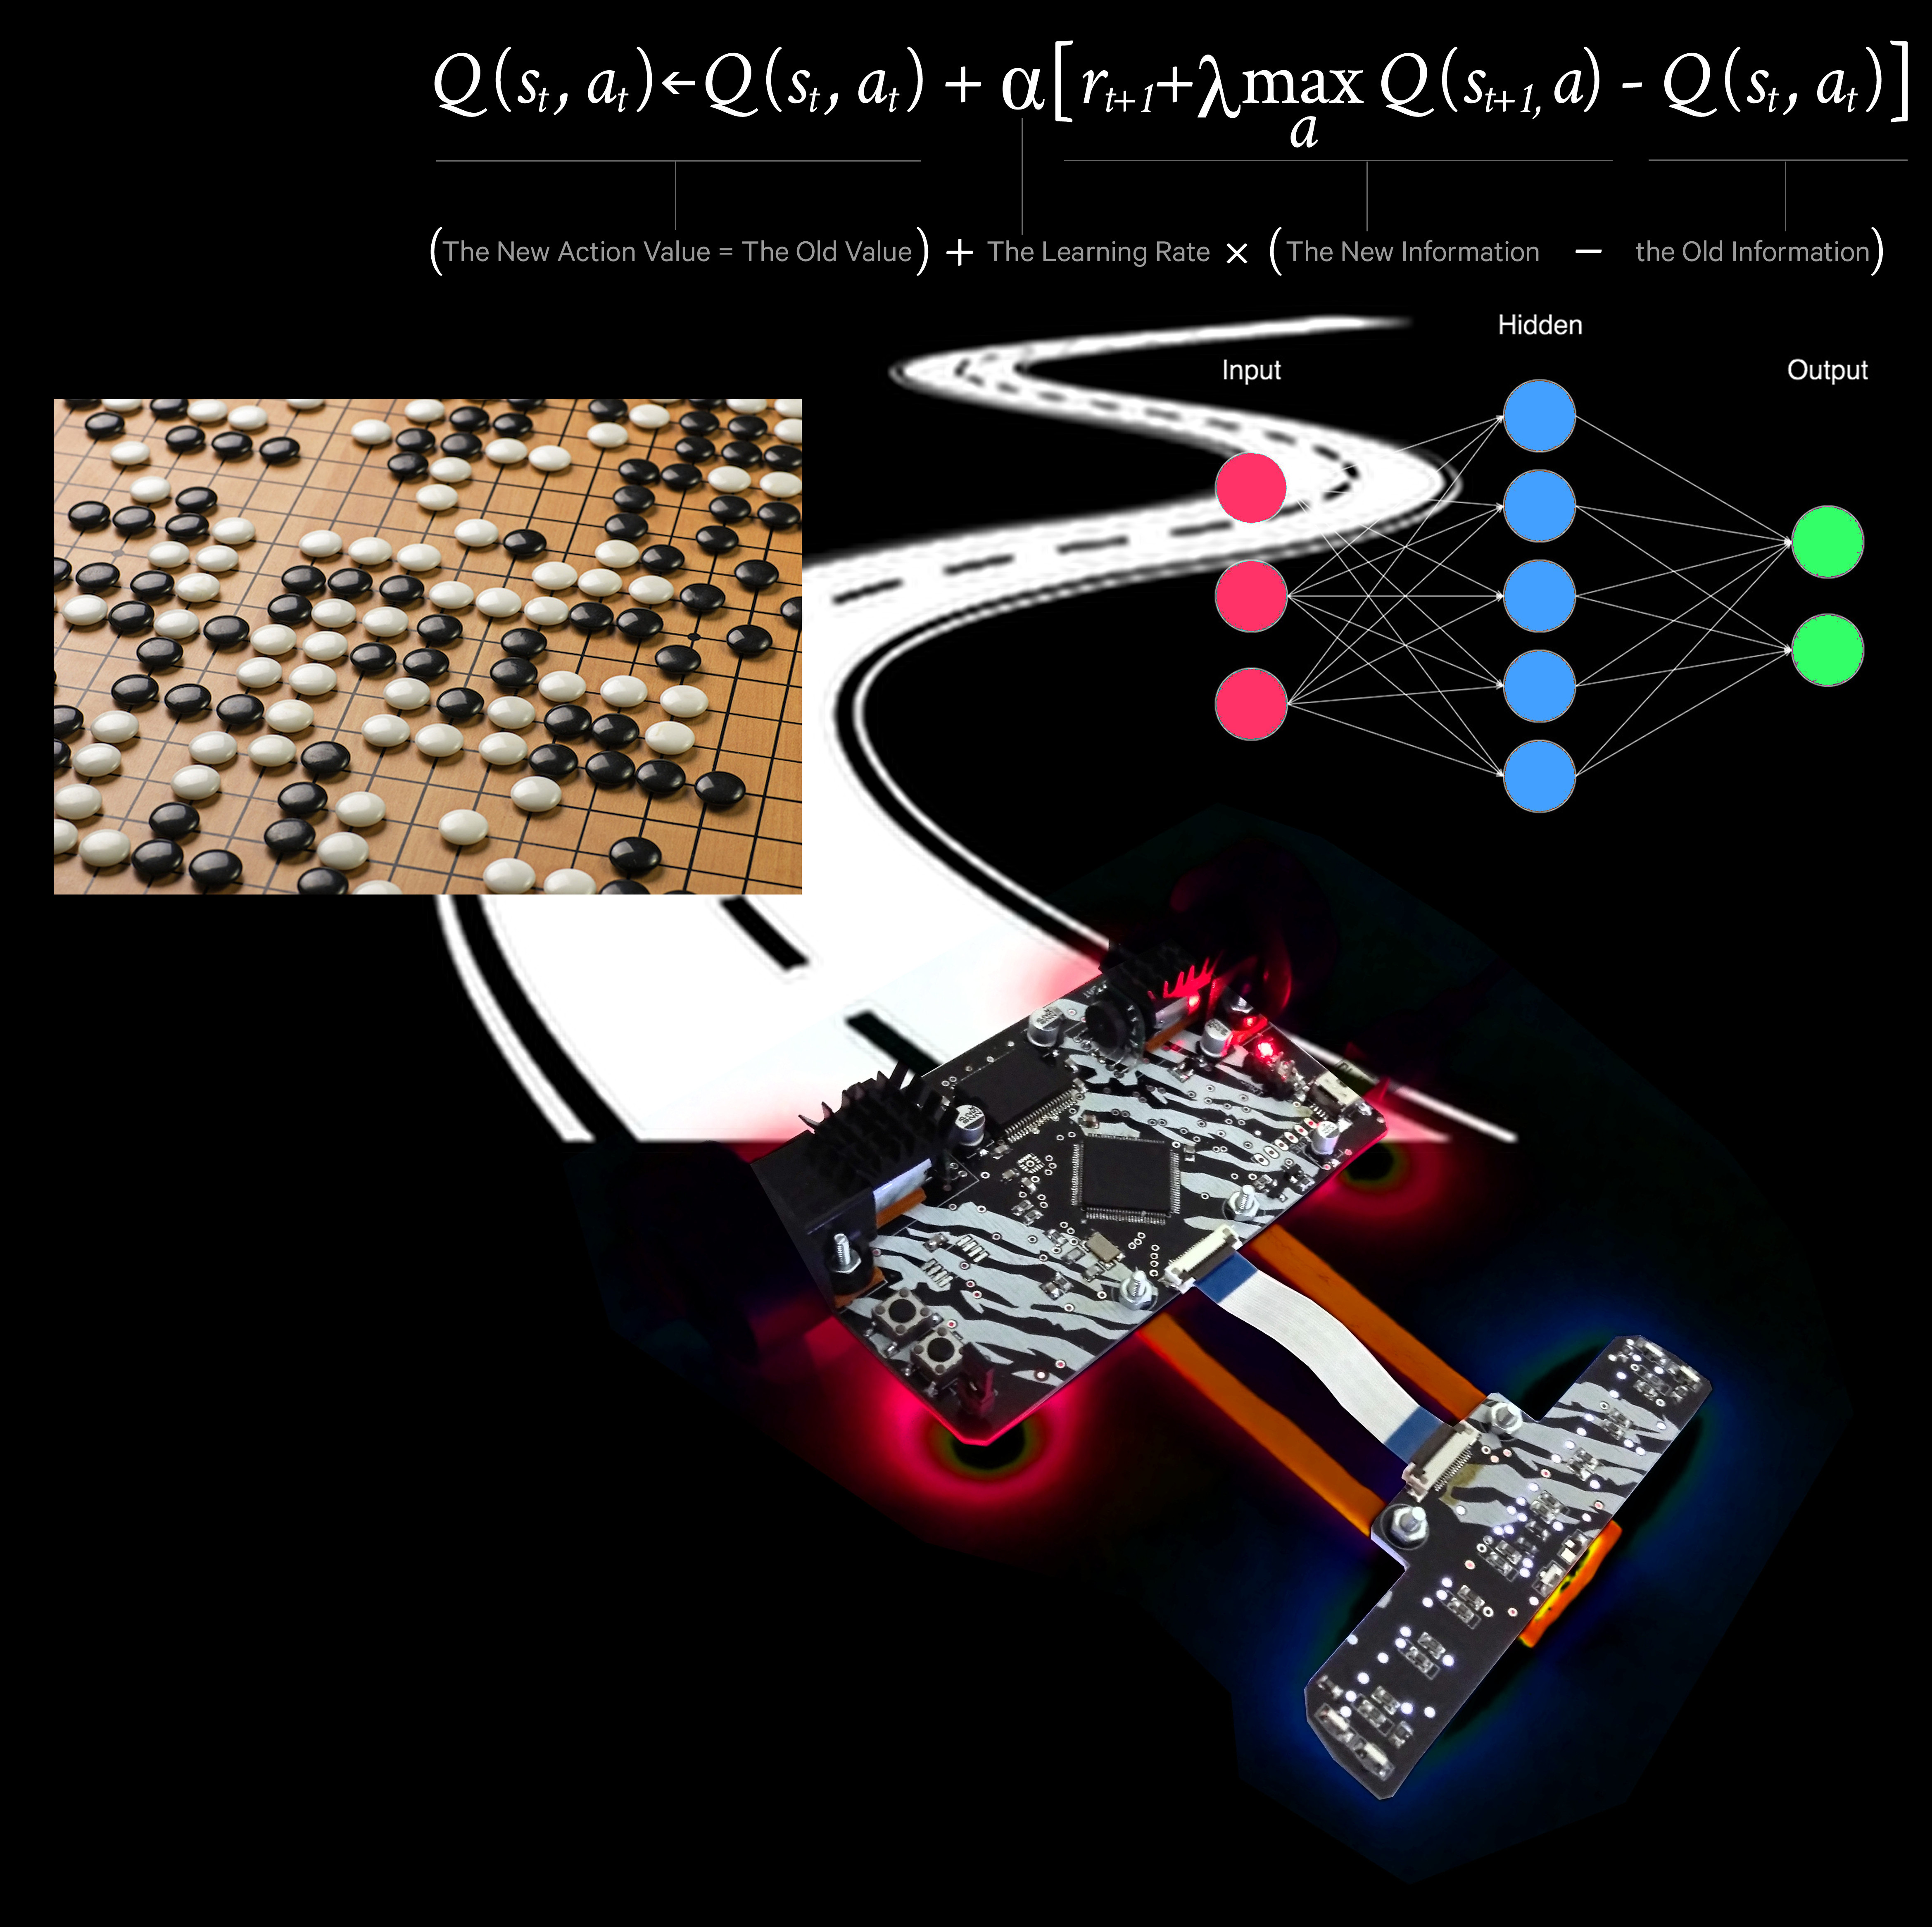
\includegraphics[width=5.05in]{../../pictures/rl_square.jpg}}

        \hfil}\vfil}
    }
    \begin{frame}

    %\titlepage


    \centering
     \colorbox{black}
     {
        \begin{minipage}{7cm}
           {\LARGE \color{white} \bf Reinforcement learning} \\
           {\LARGE \color{white} Michal CHOVANEC, PhD} \\
       \end{minipage}
     }


    \end{frame}
}


\begin{frame}{\bf Reinforcement learning}

"Master Kihara will listen to noise of fire"
\begin{figure}
  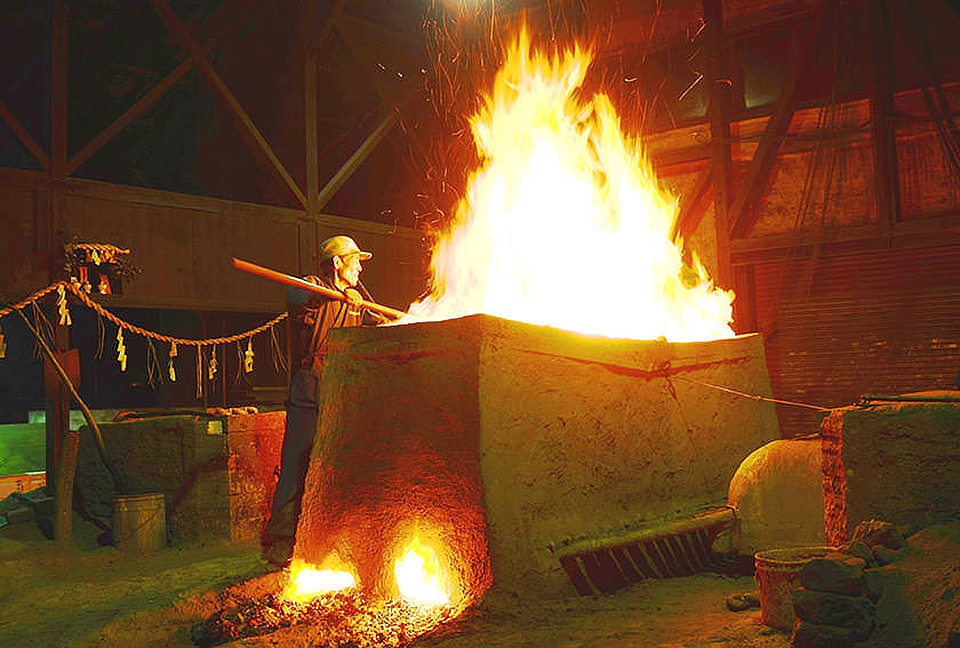
\includegraphics[scale=0.3]{../../pictures/tatara.jpg}
\end{figure}

\end{frame}


\begin{frame}{\bf Reinforcement learning}

\begin{itemize}
  \item learn from punishment and rewards
  \item learn to play a game with unknown rules
\end{itemize}

\begin{columns}
\begin{column}{0.5\textwidth}

  \begin{figure}
    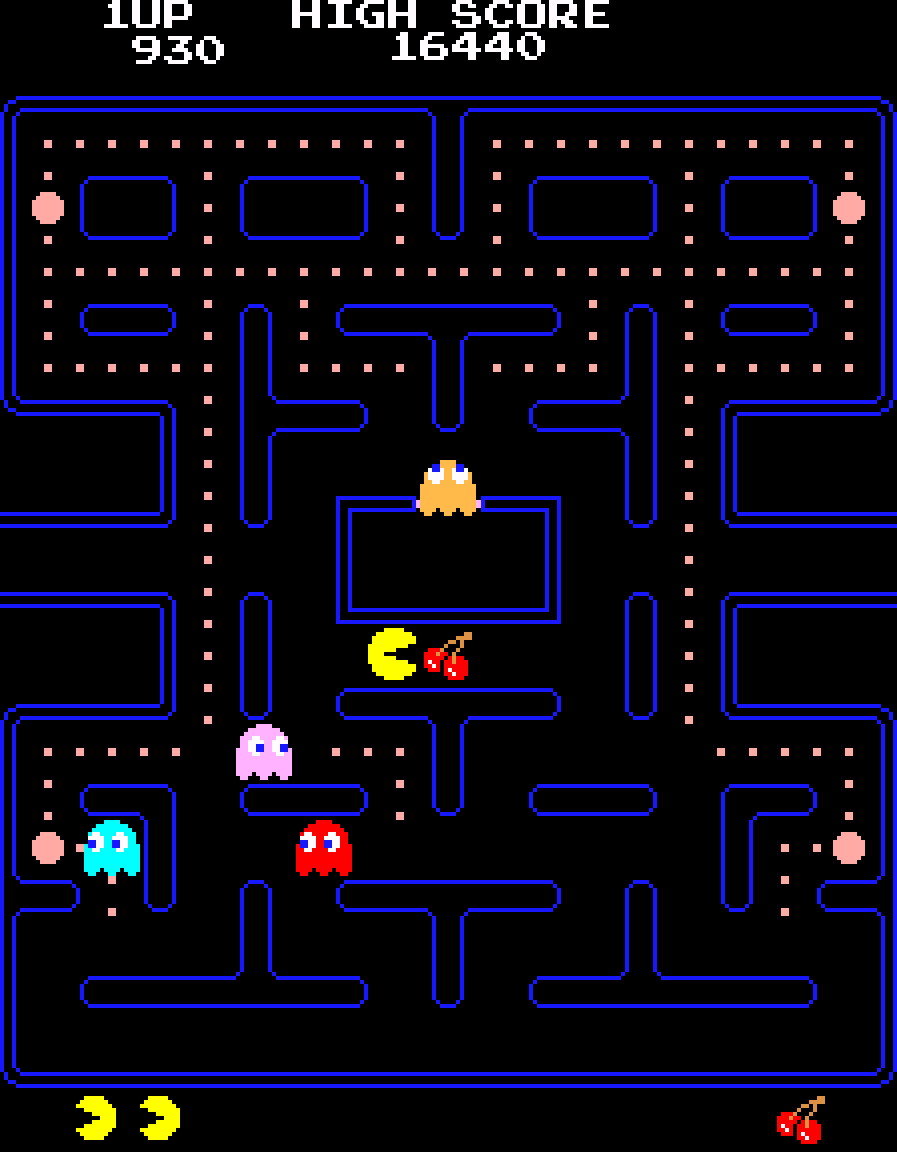
\includegraphics[scale=0.5]{../../pictures/pacman.jpg}
  \end{figure}

\end{column}
\begin{column}{0.5\textwidth}  %%<--- here

  \begin{figure}
  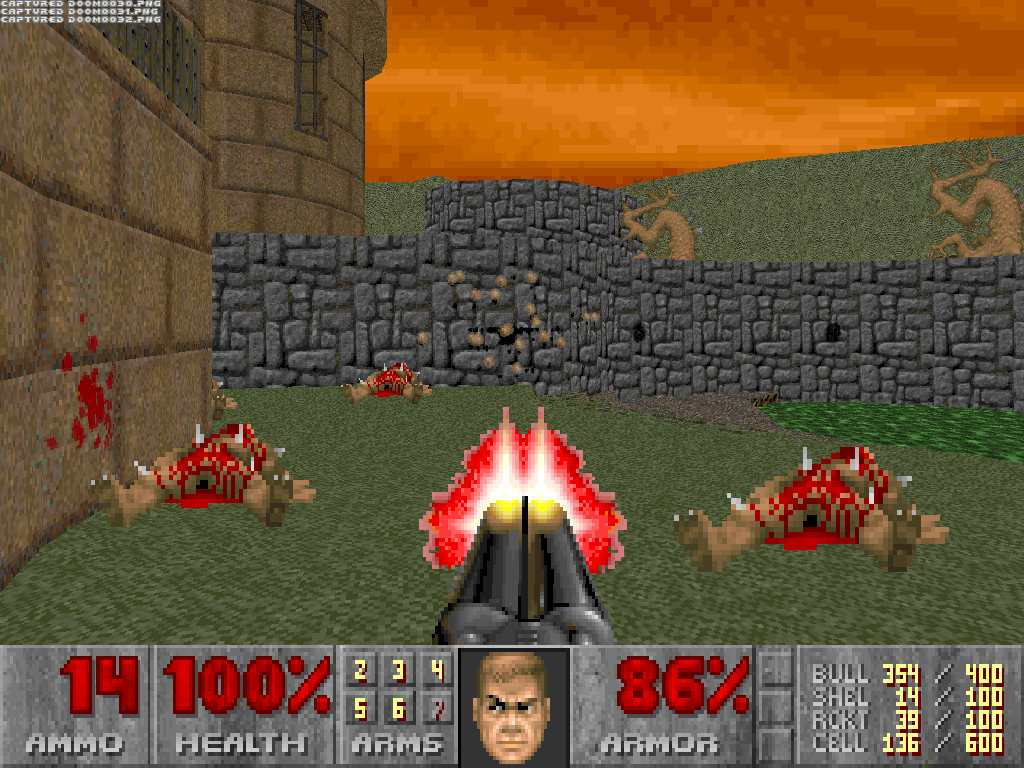
\includegraphics[scale=0.15]{../../pictures/doom.jpg}
  \end{figure}

\end{column}
\end{columns}

\vspace{-40pt}
\begin{figure}
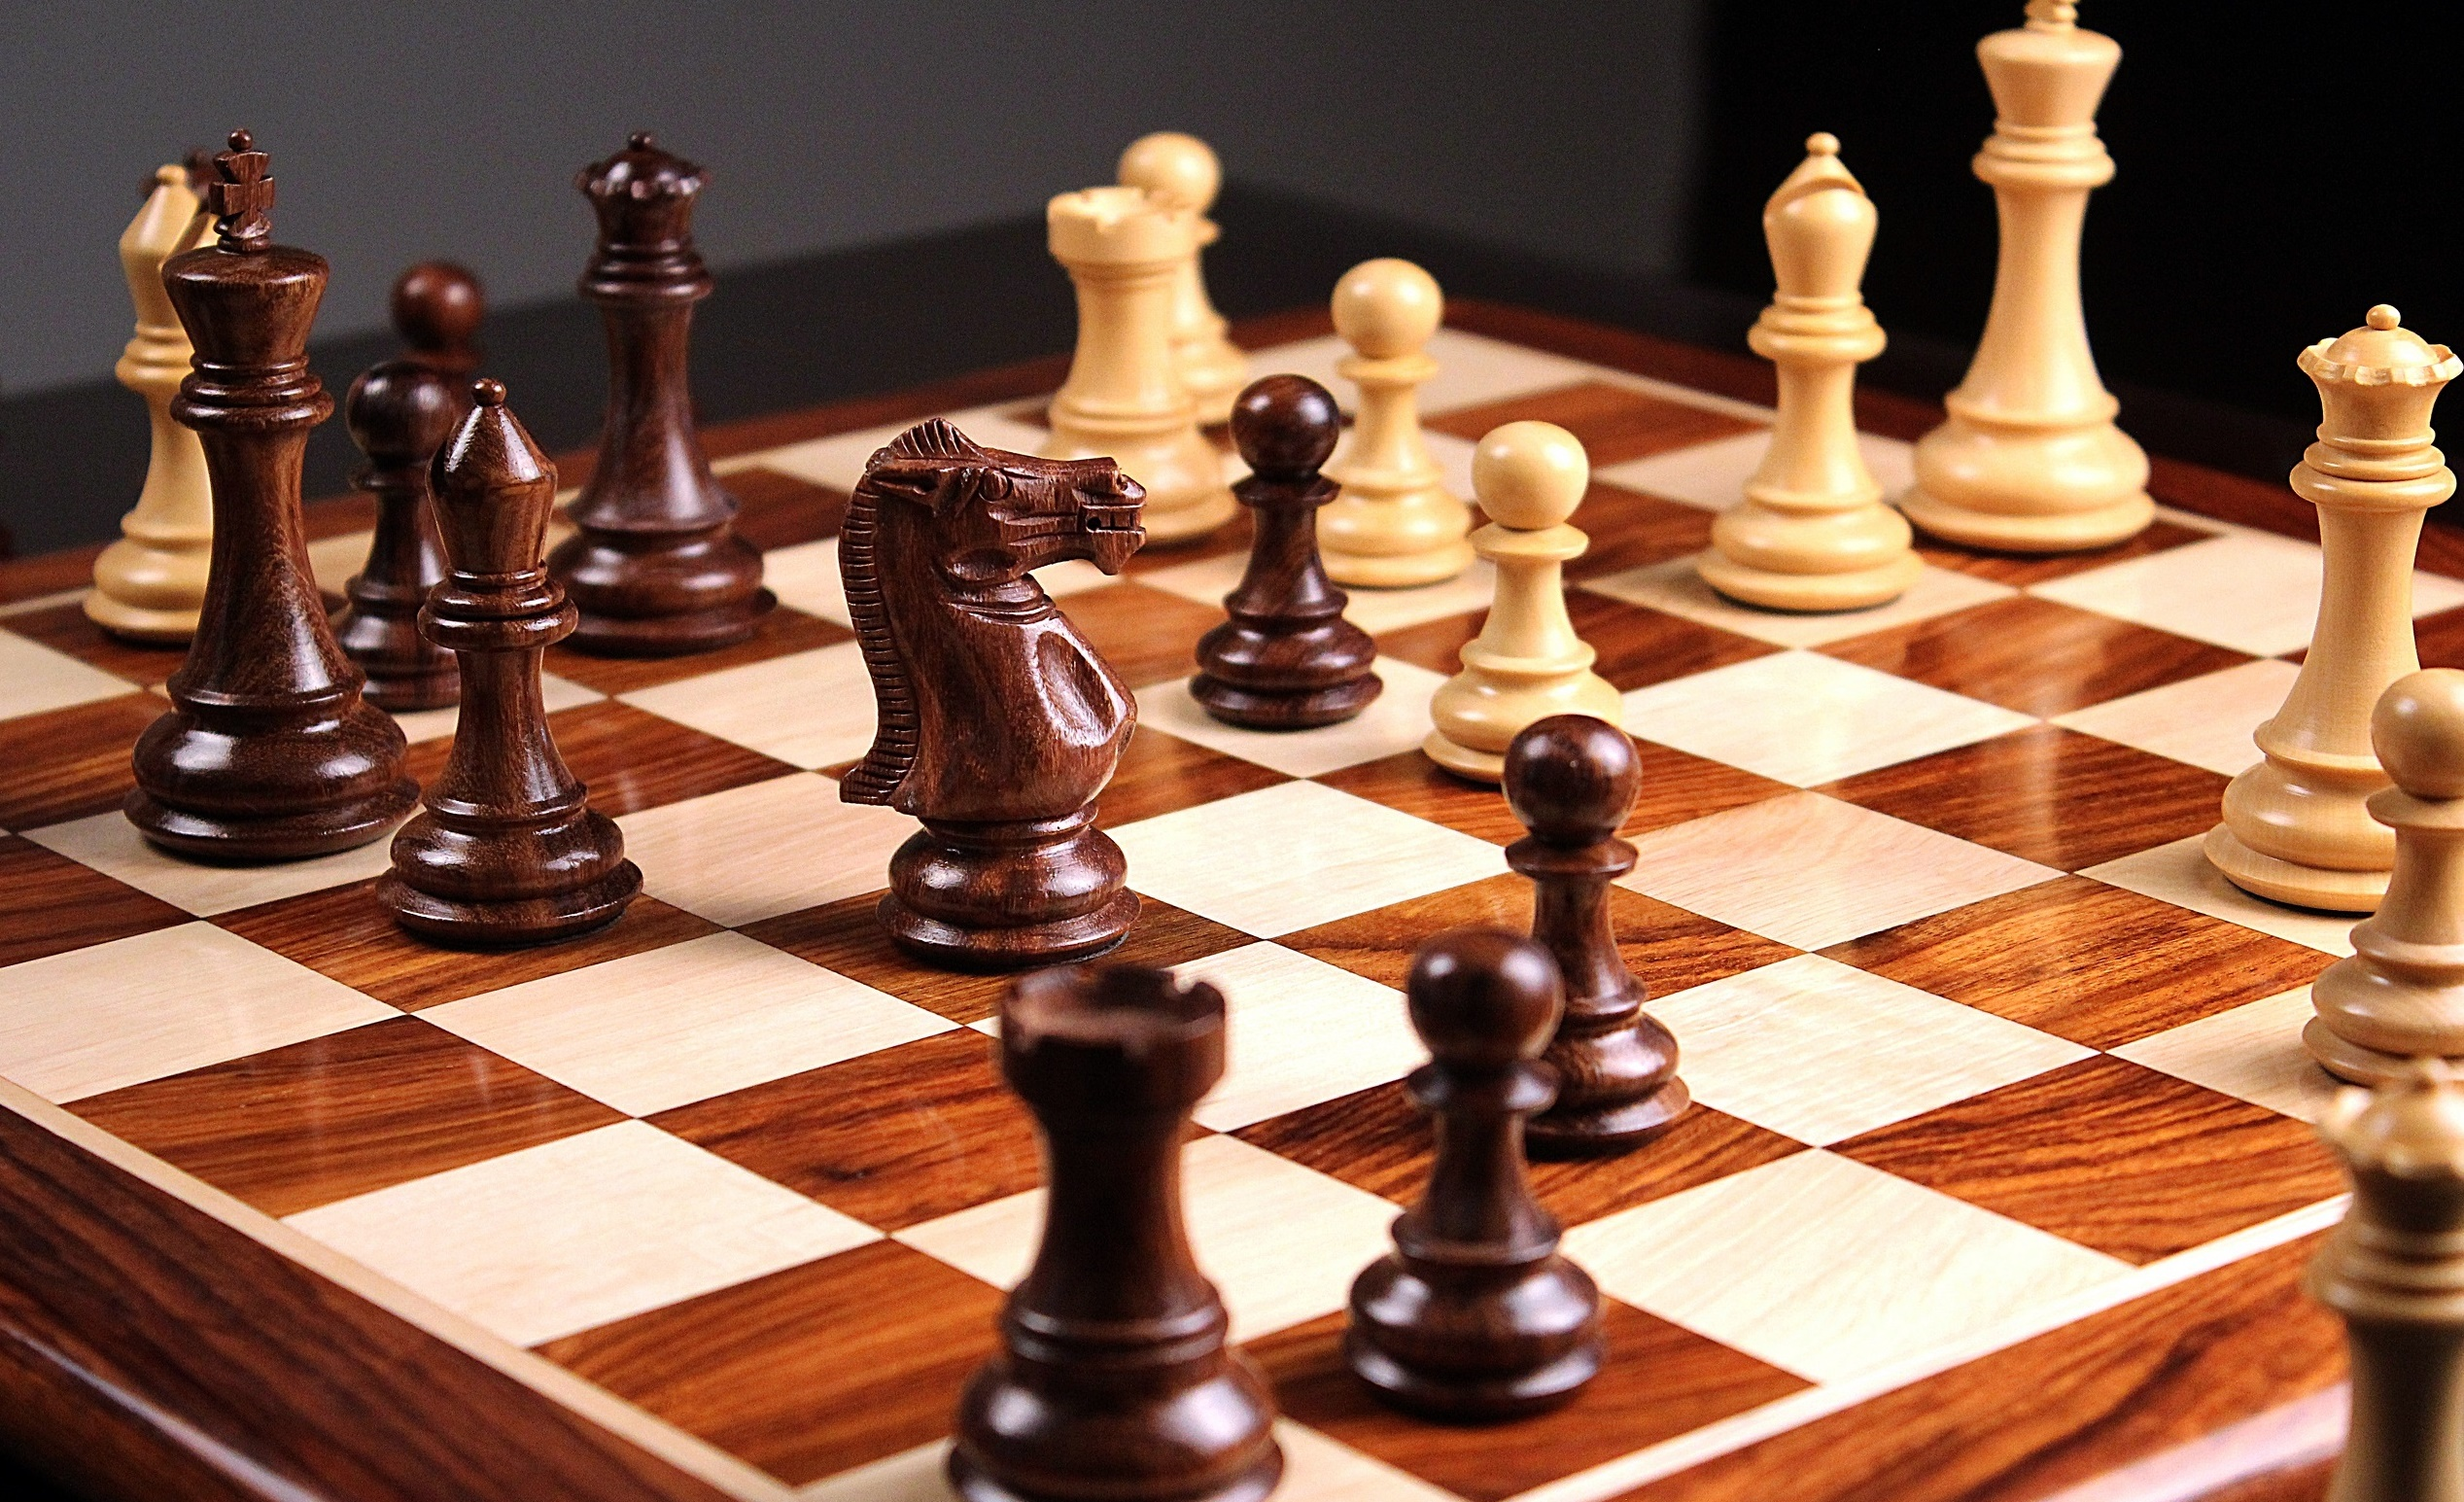
\includegraphics[scale=0.05]{../../pictures/chess.jpg}
\end{figure}

\end{frame}


\begin{frame}{\bf Reinforcement learning}


\begin{enumerate}
 \item supervised learning based on human player \\
             \begin{align*}
               action &= F(observation) \\
               loss   &= \Big(required\_action - F(observation)\Big)^2
             \end{align*}
 \item RL method \\
             \begin{align*}
               action &= F(observation) \\
               loss   &= \Big(required\_action - F(observation)\Big)^2
             \end{align*}
             {\bf \color{red} required\_action = ?} \\
             {\bf \color{green} maximize\_score}

\end{enumerate}

\end{frame}


\begin{frame}{\bf Reinforcement learning}

\begin{itemize}
  \item obtain {\bf state}
  \item choose {\bf action}
  \item {\bf execute} action
  \item obtain {\bf reward}
  \item learn from {\bf experiences}
\end{itemize}

  \begin{figure}
    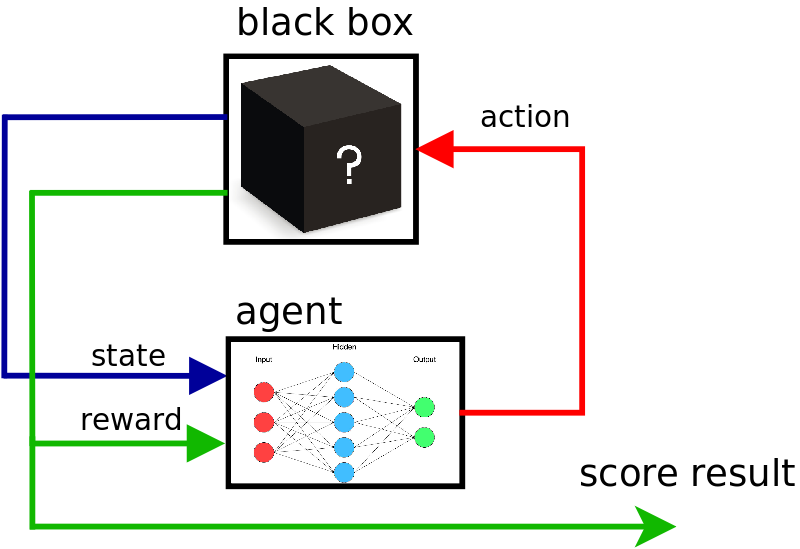
\includegraphics[scale=0.3]{../../diagrams/rl_mechanism.png}
  \end{figure}

\end{frame}

\begin{frame}{\bf Making decisions}

two possible strategies
\begin{itemize}
  \item strategy 1 : S0->S1, score = 1.0
  \item strategy 2 : S0->S2, score = 2.0
\end{itemize}

  \begin{figure}
    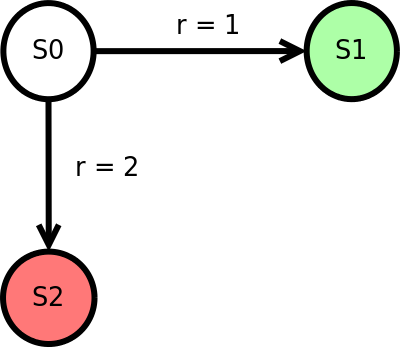
\includegraphics[scale=0.4]{../../diagrams/rl_trivial.png}
  \end{figure}

\begin{align*}
  Q(s, a) = R(s, a)
\end{align*}

where \\
  $s$ is state \\
  $a$ is action \\
  $R(s, a)$ is reward \\

\end{frame}


\begin{frame}{\bf Making decisions}

two possible strategies, {\color{red} greedy = trap}
\begin{itemize}
  \item strategy 1 : S0->S1, score = 1.0
  \item strategy 2 : S0->S2->S3, score = 2.0 + (-20.0) = -18
\end{itemize}

  \begin{figure}
    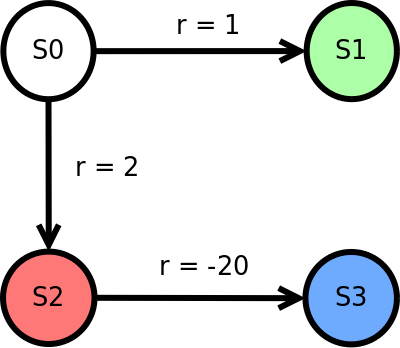
\includegraphics[scale=0.4]{../../diagrams/rl_trivial_trap.png}
  \end{figure}

  \begin{align*}
    Q(s, a) = R(s, a) + FutureReward
  \end{align*}

\end{frame}



\begin{frame}{\bf Making decisions}

three possible strategies
\begin{itemize}
  \item strategy 1 : S0->S1, score = 10.0
  \item strategy 2 : S0->S2->S3, score = -2.0 + (-20.0) = -22
  \item strategy 3 : S0->S2->S4, score = -2.0 + ( 20.0) =  18
\end{itemize}

  \begin{figure}
    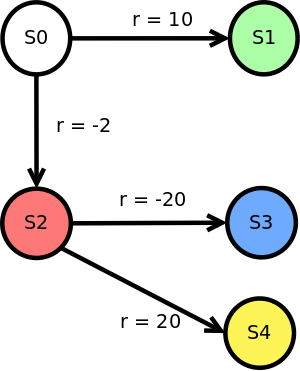
\includegraphics[scale=0.22]{../../diagrams/rl_trap.png}
  \end{figure}

  \begin{align*}
    Q(s, a) = R(s, a) + max(FutureRewards)
  \end{align*}

\end{frame}


\begin{frame}{\bf Q learning}

\begin{align*}
Q'(s, a) = R(s, a) + \gamma \max \limits_{a'} Q(s', a')
\end{align*}

where \\
$s$ is state \\
$a$ is action \\
$s'$ is next state \\
$a'$ is best action in next state \\
$R(s, a)$ is reward \\
$\gamma \in \langle 0, 1 \rangle$ is discount factor \\

\end{frame}


\begin{frame}{\bf Q learning}

\begin{align*}
Q'(s, a) = R(s, a) + \gamma \max \limits_{a'} Q(s', a')
\end{align*}

\begin{figure}
  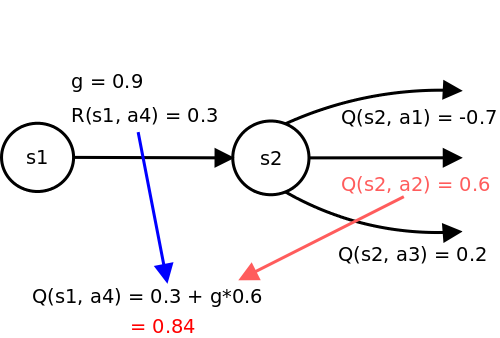
\includegraphics[scale=0.3]{../../diagrams/q_learning_detail.png}
\end{figure}

\end{frame}


\begin{frame}{\bf Q learning - stochastic}


\begin{align*}
Q'(s, a) &= R(s, a) + \gamma \max \limits_{a'} Q(s', a') \\
Q'(s, a) &= (1-\alpha)Q(s, a) + \alpha\Big(R(s, a) + \gamma \max \limits_{a'} Q(s', a')\Big)
\end{align*}


\end{frame}


\begin{frame}{\bf Q learning}

\begin{itemize}
  \item {\color{red} \bf obtain reward} \\
        reward = env.get\_reward();

  \item {\color{red} \bf update state} \\
        state\_old = state; \\
        state = env.get\_observation(); \\

  \item {\color{red} \bf select action} \\
        action\_old = action; \\
        action = select\_action(Q(state)); \\

  \item {\color{red} \bf process learning} \\
    Q(state\_old, action\_old)+= $\alpha$(reward + $\gamma$ $\max \limits_{a'}$Q(state, a') - Q(state\_old, action\_old));

  \item {\color{red} \bf execute action} \\
    env.action(action);

\end{itemize}


\end{frame}


\begin{frame}{\bf SARSA learning}

\begin{align*}
Q'(s, a) &= (1-\alpha)Q(s, a) + \alpha\Big(R(s, a) + \gamma Q(s', a')\Big)
\end{align*}

\begin{figure}
  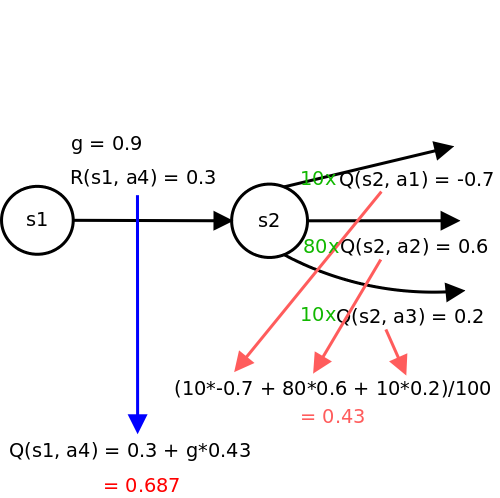
\includegraphics[scale=0.23]{../../diagrams/sarsa_learning_detail.png}
\end{figure}

\end{frame}



\begin{frame}{\bf SARSA learning}

\begin{itemize}
  \item {\color{red} \bf obtain reward} \\
        reward = env.get\_reward();

  \item {\color{red} \bf update state} \\
        state\_old = state; \\
        state = env.get\_observation(); \\

  \item {\color{red} \bf select action} \\
        action\_old = action; \\
        action = select\_action(Q(state)); \\

  \item {\color{red} \bf process learning} \\
    Q(state\_old, action\_old)+= $\alpha$(reward + $\gamma$Q(state, action) - Q(state\_old, action\_old));

  \item {\color{red} \bf execute action} \\
    env.action(action);

\end{itemize}


\end{frame}




\begin{frame}{\bf Q-learning vs SARSA - cliff example}

\begin{align*}
Q'(s, a) &= (1-\alpha)Q(s, a) + \alpha\Big(R(s, a) + \gamma \max \limits_{a'} Q(s', a')\Big) \\
Q'(s, a) &= (1-\alpha)Q(s, a) + \alpha\Big(R(s, a) + \gamma Q(s', a')\Big)
\end{align*}


\begin{figure}
  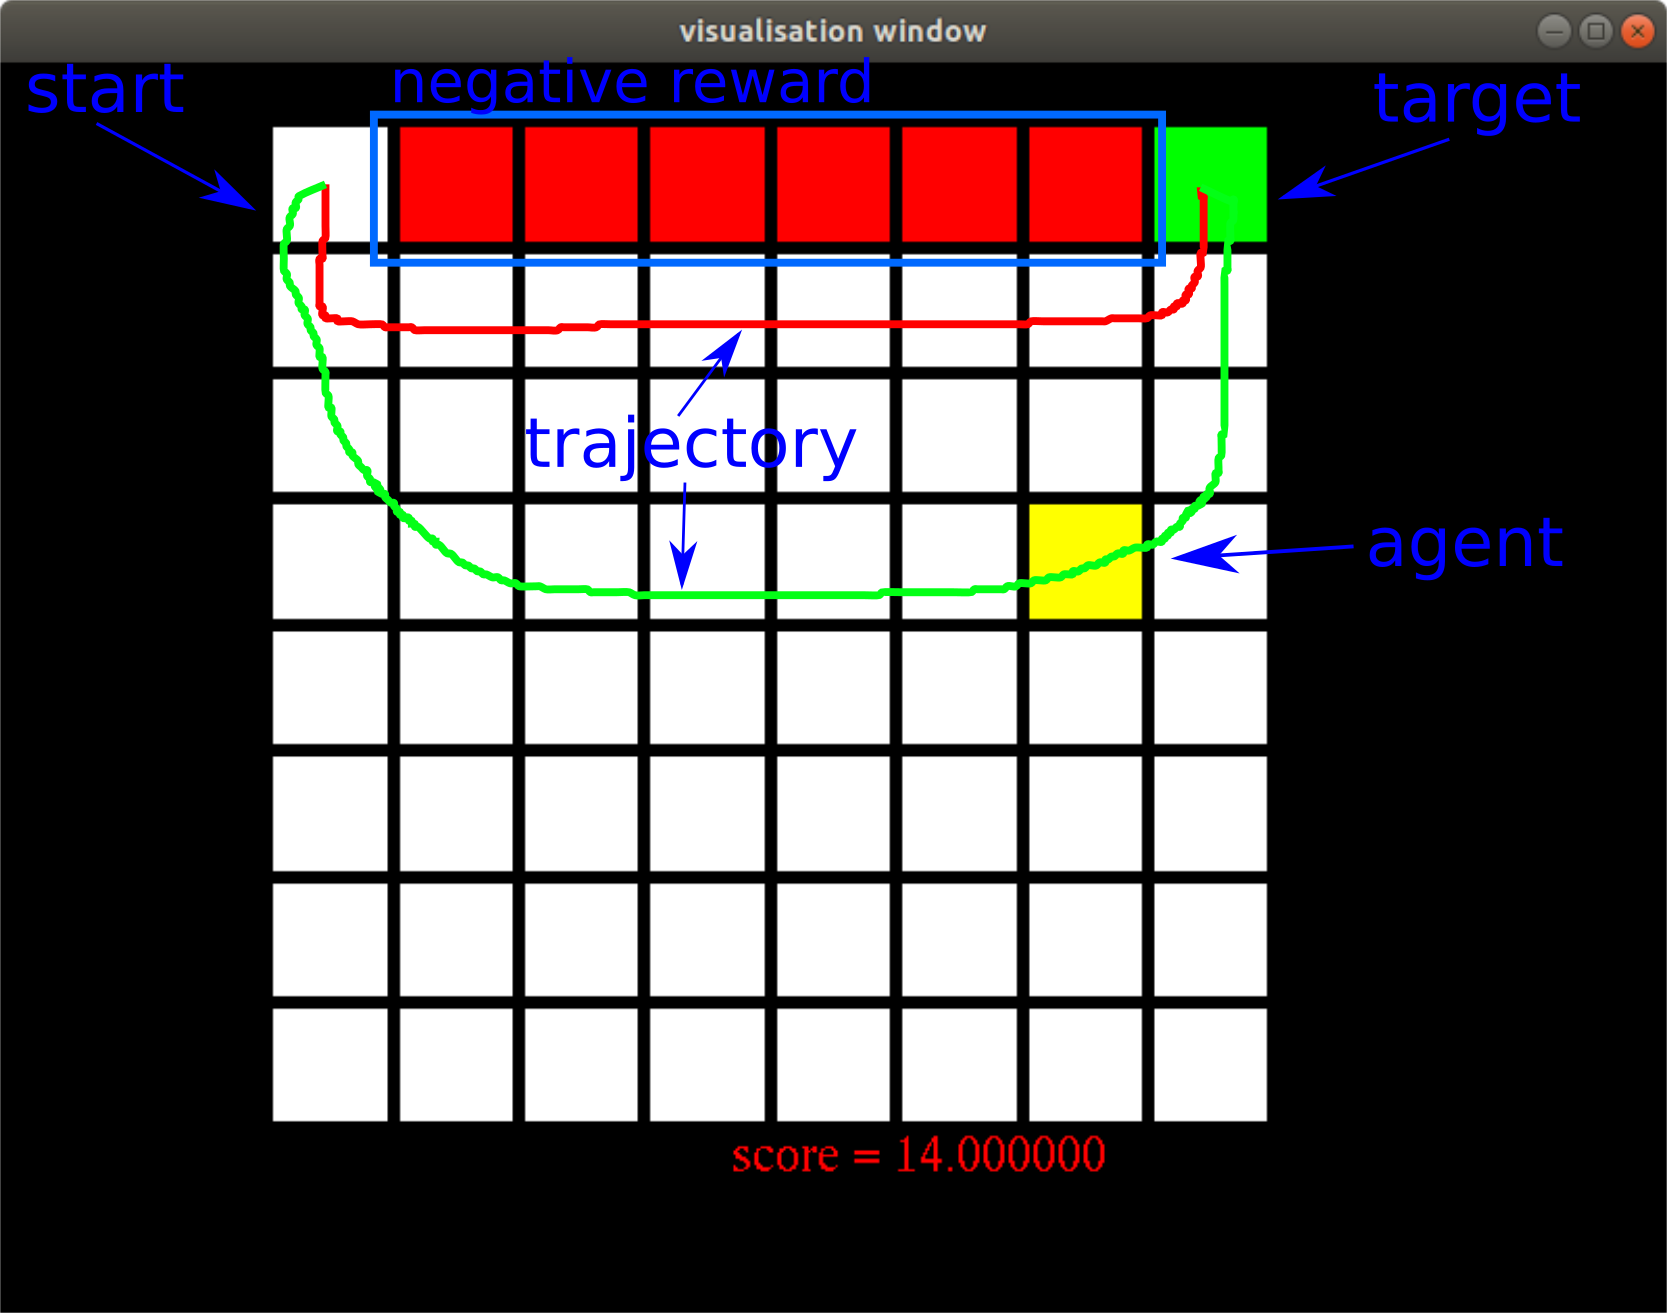
\includegraphics[scale=0.35]{../../diagrams/cliff_diagram.png}
\end{figure}

\end{frame}


\begin{frame}{\bf Deep reinforcement learning}

Possible states in some games \\

\begin{itemize}
 \item {\bf tic-tac-toe} 26830 states\\
 \item {\bf 2048}  $44 096 709 674 720 289$ states \\
 \item {\bf atoms in observable universe} $10^{82}$
 \item {\bf chess} $10^{120}$ states \\
 \item {\bf GO} $10^{170}$ states \\
\end{itemize}

% 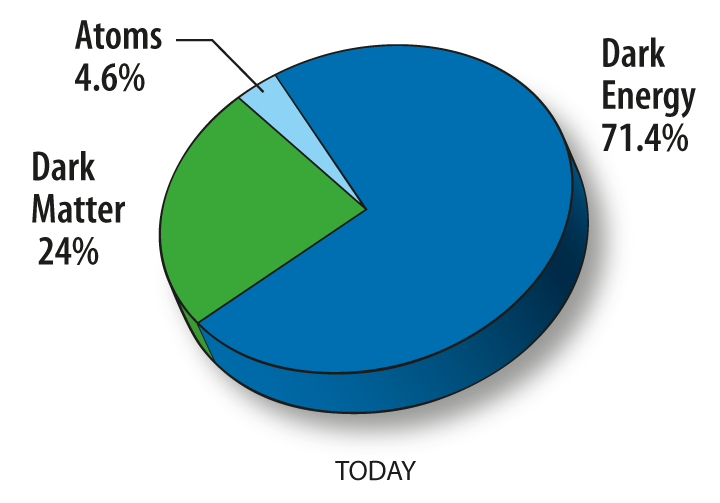
\includegraphics[scale=0.1]{../../pictures/universe_atoms.png} \\

storing Q values

\begin{itemize}
 \item table \\
 \item linear combination of features, $ Q(s, a) = \sum_{i=1}^{N} w_iF_i(s, a) $
 \item neural network
\end{itemize}


\end{frame}



\begin{frame}{\bf Q table example}

\begin{figure}
  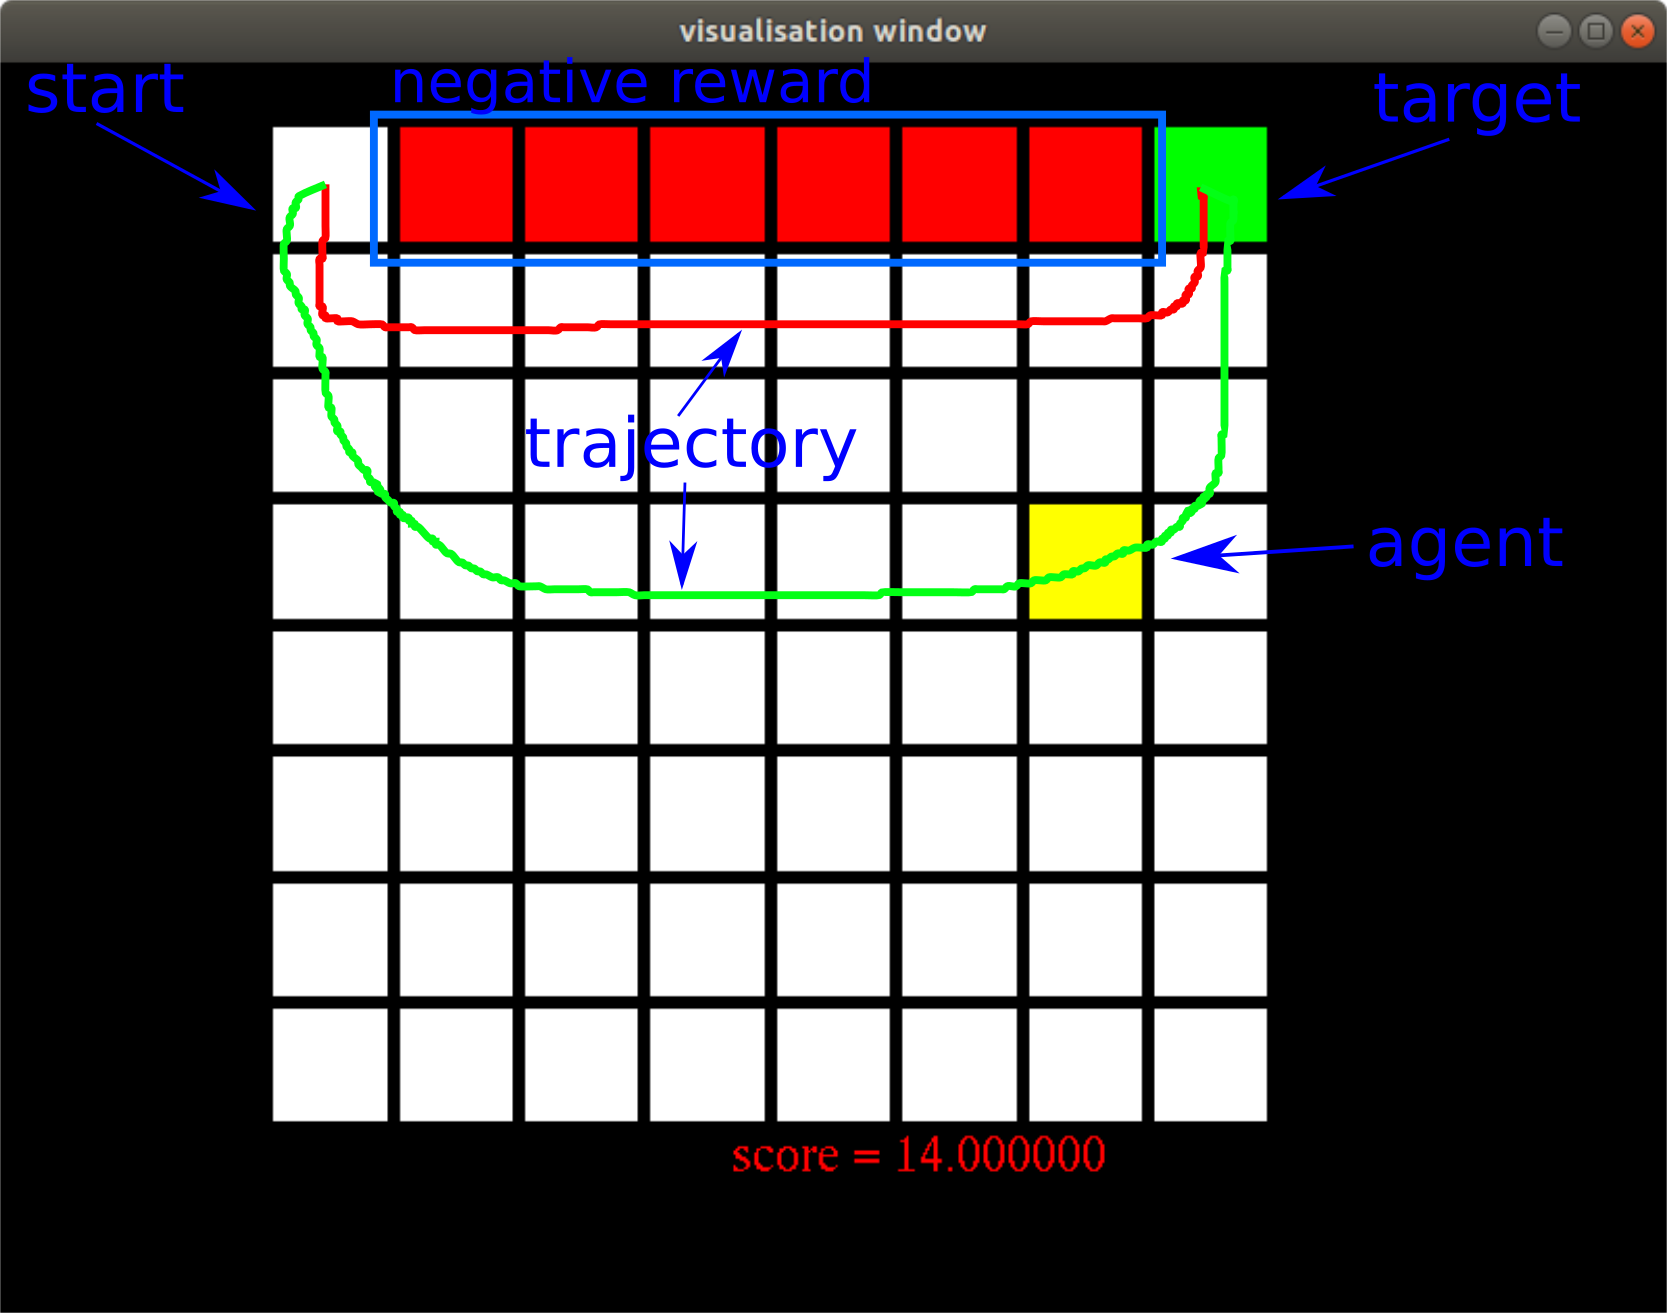
\includegraphics[scale=0.2]{../../diagrams/cliff_diagram.png}
\end{figure}

{\tiny
  \begin{table}[]
  \begin{tabular}{|l|l|l|l|l|}
  \hline
  \textbf{State}                                              & \textbf{A0 UP}                    & \textbf{A1 LEFT} & \textbf{A2 DOWN} & \textbf{A3 RIGHT}         \\ \hline
  0                                                           &                                   &                  & 0.43             & {\color[HTML]{FE0000} -1} \\ \hline
  \begin{tabular}[c]{@{}l@{}}1, 2, 3, \\ 4, 5, 6\end{tabular} & \textbf{T}                        & \textbf{T}       & \textbf{T}       & \textbf{T}                \\ \hline
  7                                                           & \textbf{T}                        & \textbf{T}       & \textbf{T}       & \textbf{T}                \\ \hline
  8                                                           &                                   &                  &                  & 0.49                      \\ \hline
  9                                                           & {\color[HTML]{FE0000} -1}         &                  &                  & 0.53                      \\ \hline
  10                                                          & {\color[HTML]{FE0000} -1}         &                  &                  & 0.59                      \\ \hline
  11                                                          & {\color[HTML]{FE0000} -1}         &                  &                  & 0.65                      \\ \hline
  12                                                          & {\color[HTML]{FE0000} -1}         &                  &                  & 0.72                      \\ \hline
  13                                                          & {\color[HTML]{FE0000} -1}         &                  &                  & 0.81                      \\ \hline
  14                                                          & {\color[HTML]{FE0000} -1}         &                  &                  & 0.9                       \\ \hline
  \textbf{15}                                                 & {\color[HTML]{34FF34} \textbf{1}} &                  &                  &                           \\ \hline
  \end{tabular}
  \end{table}
}

\end{frame}




\begin{frame}{\bf Neural network for $Q(s, a)$ approximation - \\ Q networks}

\centering
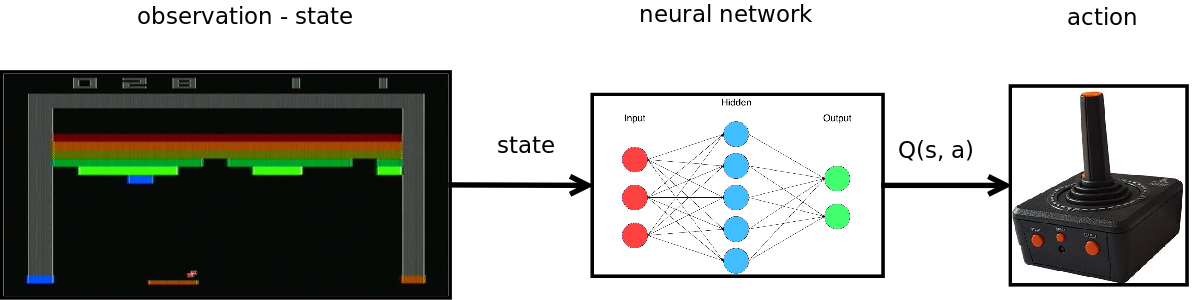
\includegraphics[scale=0.18]{../../diagrams/q_net.png}

\end{frame}

\begin{frame}{\bf Neural network for $Q(s, a)$ approximation - \\ Q networks}

\centering
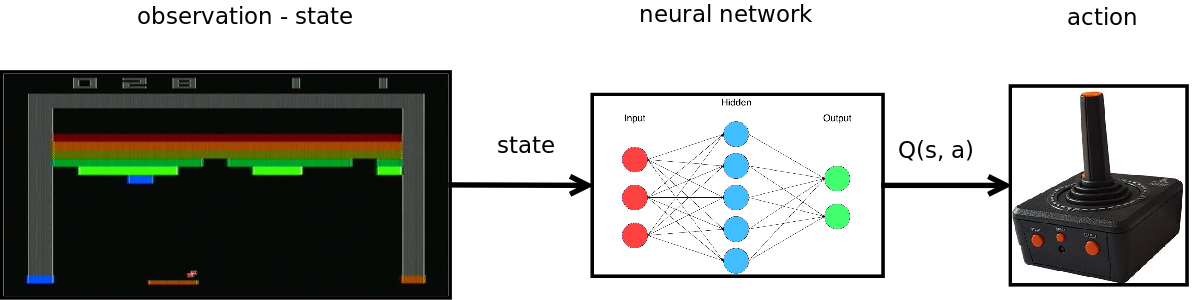
\includegraphics[scale=0.13]{../../diagrams/q_net.png}

\begin{align*}
SARSA : Q'(s, a) &= (1-\alpha)Q(s, a) + \alpha\Big(R(s, a) + \gamma Q(s', a')\Big)
\end{align*}
\begin{align*}
  loss   &= \sum_{i=1}^{N} \Big(target\_value_i - resulted\_value_i\Big)^2 \\
  L   &= \sum_{i=1}^{N} \Big(Q(s_i, a_i) - \hat{Q}(s_i, a_i)\Big)^2 \\
  L   &= \sum_{i=1}^{N} \Big(R(s_i, a_i) + \gamma Q(s'_i, a_i') - \hat{Q}(s_i, a_i)\Big)^2
\end{align*}

\end{frame}





\begin{frame}{\bf Training network}

\begin{columns}
  \begin{column}{0.5\textwidth}

      \begin{figure}
        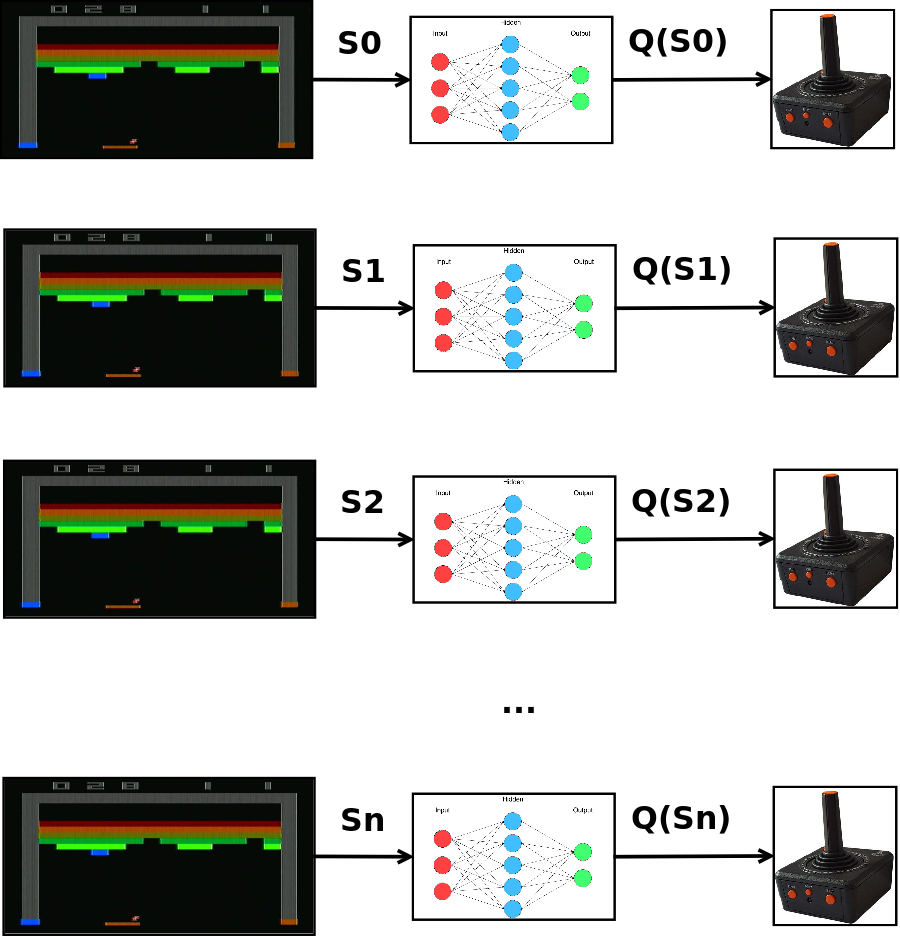
\includegraphics[scale=0.12]{../../diagrams/q_net_unrolled.png}
      \end{figure}

  \end{column}
  \begin{column}{0.5\textwidth}  %%<--- here

      \begin{align*}
        \Delta \hat{Q} (s_0, a_0) &= \alpha\Big(R(s_0, a_0) + \gamma \hat{Q}(s_1, a_1)\Big) \\
        \Delta \hat{Q}(s_1, a_1) &= \alpha\Big(R(s_1, a_1) + \gamma \hat{Q}(s_2, a_2)\Big) \\
        \Delta \hat{Q}(s_2, a_2) &= \alpha\Big(R(s_2, a_2) + \gamma \hat{Q}(s_3, a_3)\Big) \\
        ... \\
        \Delta \hat{Q}(s_{n}, a_{n}) &= \alpha\Big(R(s_{n}, a_{n}) + \gamma \hat{Q}(s_{n+1}, a_{n+1})\Big)
      \end{align*}

  \end{column}
\end{columns}


\end{frame}


\begin{frame}{\bf Training network}

\begin{enumerate}
\item compute temporary $Q_t$ batch
      \begin{align*}
        Q_t (s_0, a_0) &= R(s_0, a_0) + \gamma Q_t(s_1, a_1) \\
        Q_t(s_1, a_1) &= R(s_1, a_1) + \gamma Q_t(s_2, a_2) \\
        Q_t(s_2, a_2) &= R(s_2, a_2) + \gamma Q_t(s_3, a_3) \\
        ... \\
        Q_t(s_n, a_n) &= R(s_{n+1}, a_{n+1})
      \end{align*}

\item train neural network using
      \begin{align*}
        Q_{new}(s_i, a_i) &= (1 - \alpha)Q_{old}(s_i, a_i) + \alpha Q_t(s_i, a_i)
      \end{align*}

\end{enumerate}


\end{frame}


\begin{frame}{\bf Examples}


\begin{figure}
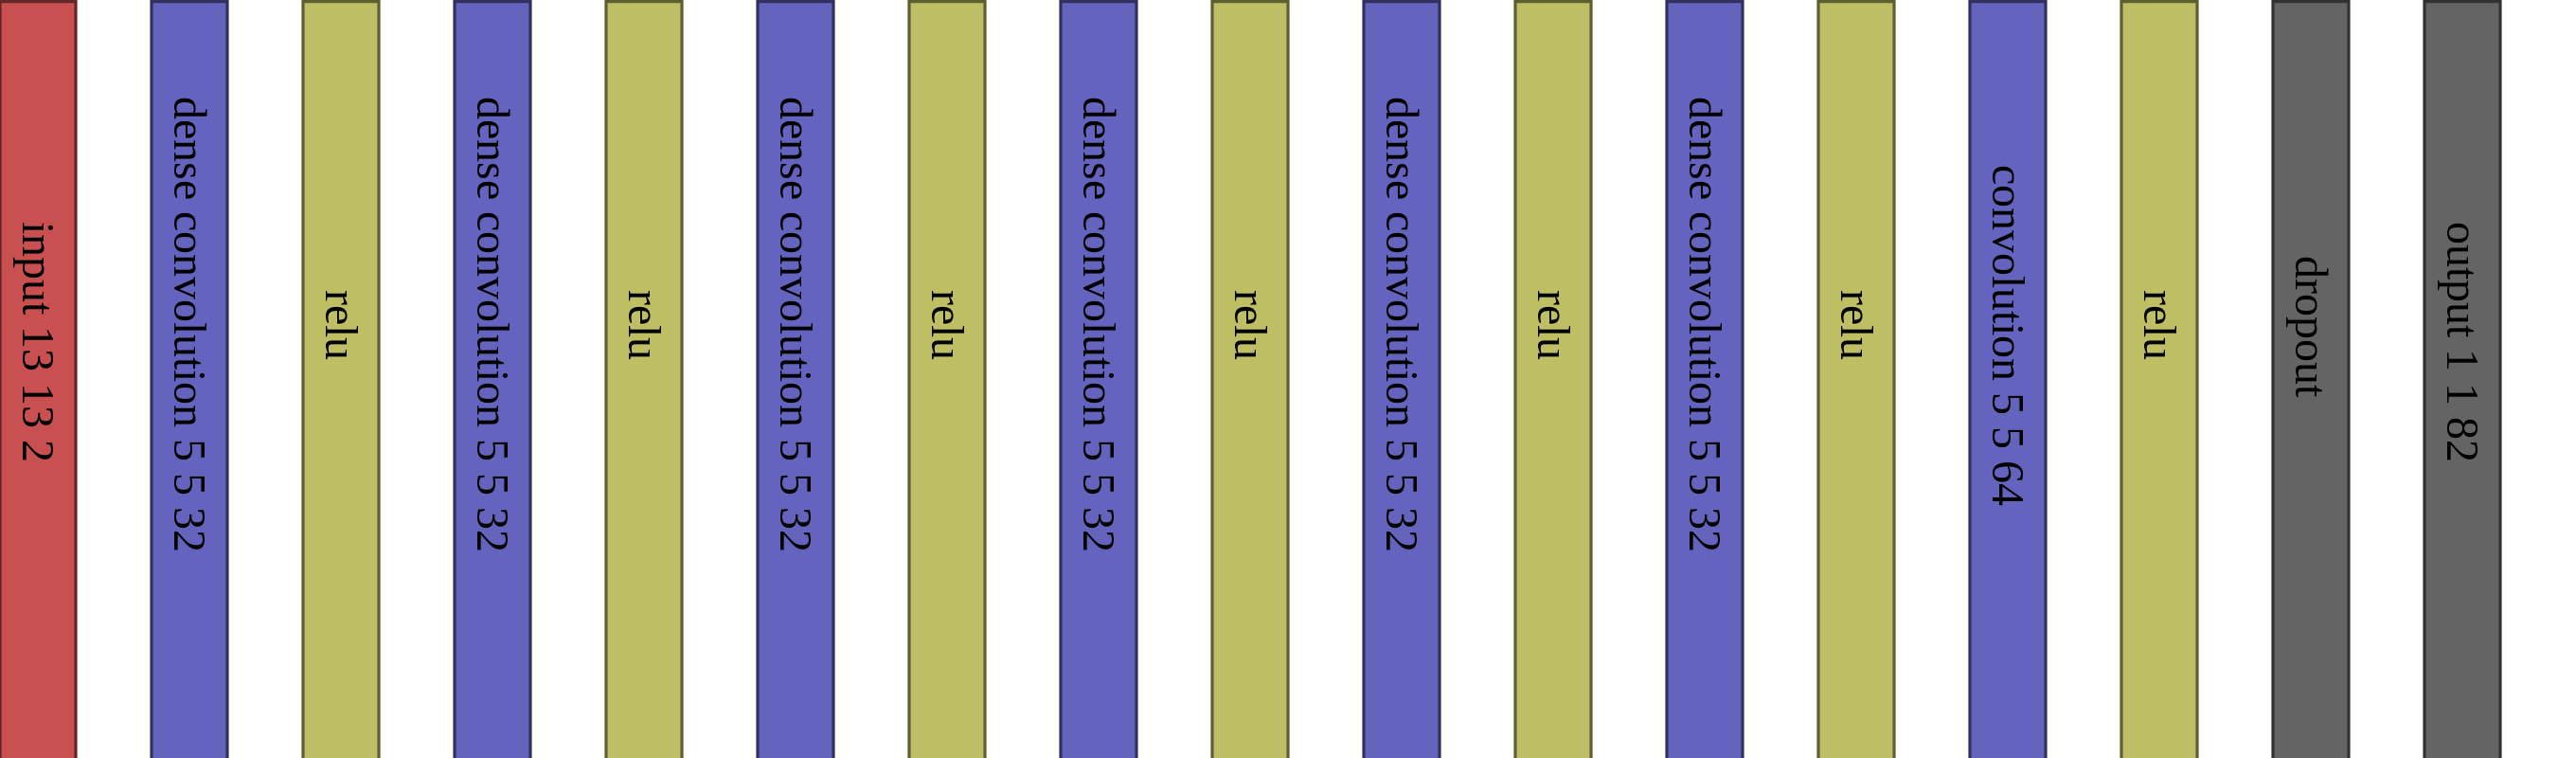
\includegraphics[scale=0.11]{../../pictures/go_cnn_architecture.png}
\end{figure}

\begin{columns}
\begin{column}{0.5\textwidth}

  \begin{figure}
    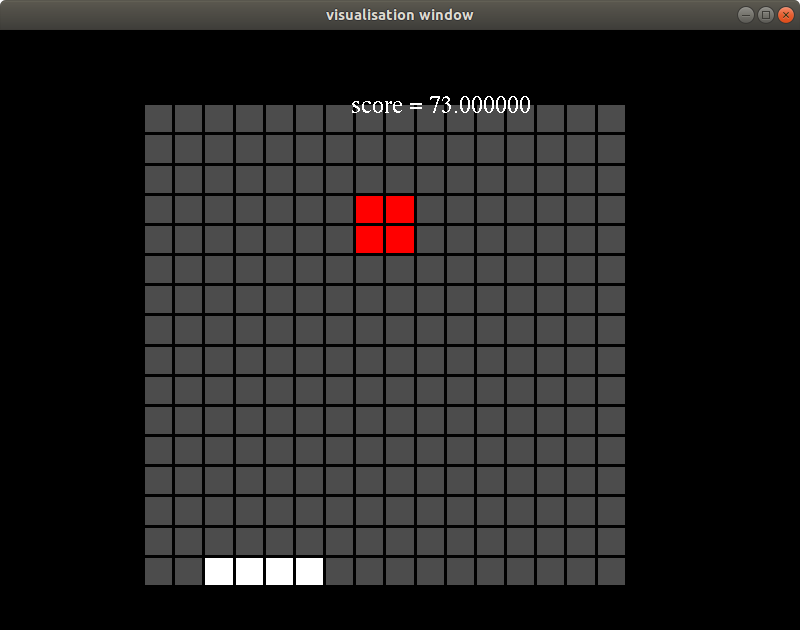
\includegraphics[scale=0.18]{../../pictures/catcher.png}
  \end{figure}

\end{column}
\begin{column}{0.5\textwidth}  %%<--- here

  \begin{figure}
  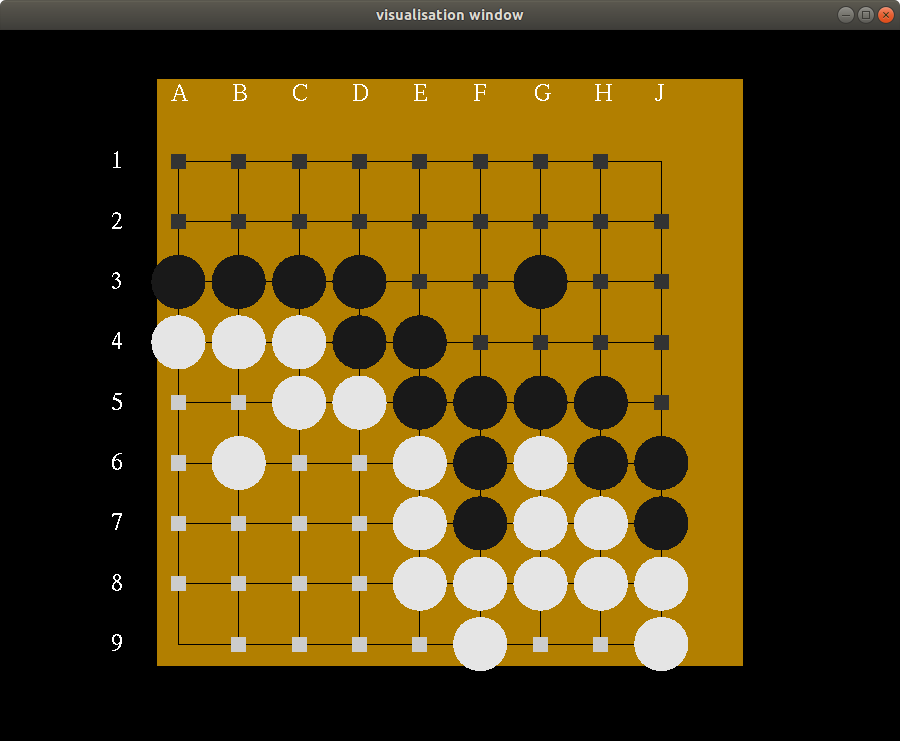
\includegraphics[scale=0.19]{../../pictures/go.png}
  \end{figure}

\end{column}
\end{columns}



\end{frame}




\begin{frame}{\bf Usefull links}

{\tiny
  \begin{thebibliography}{9}
    \bibitem {}Andrej Karpathy : Pong from pixels \\ \url{http://karpathy.github.io/2016/05/31/rl/}
    \bibitem {}Richard S. Sutton : Reinforcement Learning: An Introduction \\ \url{https://www.amazon.com/Reinforcement-Learning-Introduction-Adaptive-Computation/dp/0262193981}
    \bibitem {}Maxim Lapan : Deep reinforcement learning \\ \url{https://www.amazon.com/Practical-Reinforcement-Learning-Maxim-Lapan/dp/1788834240}
    \bibitem {}Mohit Sewak : Practical Convolutional Neural \\ Networks \url{https://www.amazon.com/Practical-Convolutional-Neural-Networks-Implement/dp/1788392302}
    \bibitem {}CHRISTOPHER  J.C.H. WATKINS : Q-learning \\ \url{http://www.gatsby.ucl.ac.uk/~dayan/papers/cjch.pdf}
    \bibitem {}Densely Connected Convolutional Networks \\ \url{https://arxiv.org/pdf/1608.06993.pdf}
    \bibitem {}Mastering the Game of Go without Human Knowledge \\ \url{https://deepmind.com/documents/119/agz_unformatted\_nature.pdf}
  \end{thebibliography}
}

\end{frame}


\begin{frame}{\bf Q\&A}

\begin{figure}
  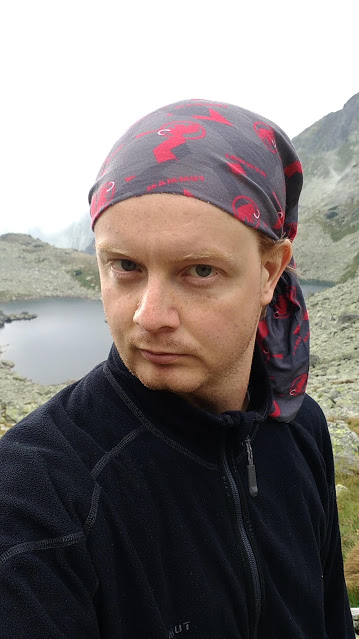
\includegraphics[scale=0.25]{../../pictures/me.jpg}
\end{figure}

\centering {
michal chovanec (michal.nand@gmail.com)
\url{www.youtube.com/channel/UCzVvP2ou8v3afNiVrPAHQGg}
}

\centering {
github
\url{https://github.com/michalnand}
}

\end{frame}


\end{document}
